\chapter{NFC tehnologija}
NFC je tehnologija dvosmjernog be\v{z}i\v{c}nog prijenosa podataka izme\dj u dva ure\dj aja u kratkom dometu. NFC je osmi\v{s}ljen da korisnicima pru\v{z}i siguran, brz i jednostavan pristup digitalnom sadr\v{z}aju, uparivanje ure\dj aja i beskontaktne transakcije.

Kao protokol posebno je zanimljiv industriji pametnih telefona jer su NFC moduli kompaktni i cjenovno pristupa\'{c}ni. Po\v{s}to ve\'{c}ina ljudi danas posjeduje pametni telefon, a samim tim i NFC ure\dj aj, razni proizvo\dj a\v{c}i mobilnih aplikacija implementiraju NFC povezivost u svoje aplikacije te time pro\v{s}iruju domenu funkcionalnosti koje nude svojim korisnicima. Primjer je mobilna aplikacija Foursquare \cite{foursquare} koja koriste\'{c}i NFC omogu\'{c}uje korisnicima da se prijave na razim mjestima interesa (POI) kao \v{s}to su restorani, hoteli, ulice... Kada korisnik pre\dj e pametnim telefonom do 10 cm iznad naljepnice aplikacija, koriste\'{c}i NFC senzor, skenira podatke o lokaciji POI-a koje u svojoj memoriji sadr\v{z}i NFC ure\dj aj. Logo Forsquare-a je prikazan na slici  ~\ref{fig:forsquare}.

\begin{figure}[!htbp]
	\begin{center}
 
\includegraphics[height=6cm,keepaspectratio=true]{nfc_forsquare}
 \caption{Logo aplikacije Forsquare \cite{foursquare}}
 \label{fig:forsquare}
	\end{center}
\end{figure}

2004. godine je osnovano neprofitno dru\v{s}tvo NFC Forum \cite{nfc_forum} \v{c}iji \v{c}lanovi uklju\v{c}uju firme koje se bave razvojem i primjenom NFC-a u svim segmentima tehnologije. Cilj dru\v{s}tva je razvoj i standardizacija protokola i ure\dj aja koji ga koriste. NFC Forum su osnovale tvrtke Sony, Nokia i NPX Semiconductors, te dru\v{s}tvo danas broji preko 190 \v{c}lanova. Neki od \v{c}lanova su vode\'{c}e svjetske tehnolo\v{s}ke kompanije, kao npr. Apple, Google, Intel i Samsung. Na slici  ~\ref{fig:nfc} je prikazan logotip protokola.

\begin{figure}[!htbp]
	\begin{center}
 
\includegraphics[height=4cm,keepaspectratio=true]{nfc_logo}
 \caption{Logo NFC protokola \cite{nfc_forum}}
 \label{fig:nfc}
	\end{center}
\end{figure}

\section{Arhitektura}

NFC komunikacija se sastoji od dva ure\dj aja koja u sebi sadr\v{z}e antene u obliku zavojnice:
\begin{itemize}
	\item Ure\dj aj koji inicira komunikaciju
	\item Ure\dj aj koji slu\v{s}a i \v{c}eka da komunikacija bude inicirana
\end{itemize}

Komunikacija se vr\v{s}i preko magnetskog polja koje se stvara izme\dj u antena, sli\v{c}no kao kod elektri\v{c}nog transformatora \cite{nfc_techonology}. Komunikacija se vr\v{s}i na frekvenciji od 13.56 MHz i brzine je do 424 kbit/s. Maksimalna udaljenost izme\dj u dva ure\dj aja koja komuniciraju je 4 cm\textsuperscript{3}. Na slici ~\ref{fig:nfc_arhitektura} su prikazana oba ure\dj aja te magnetsko polje izme\dj u njih.


\begin{figure}[!htbp]
	\begin{center}
 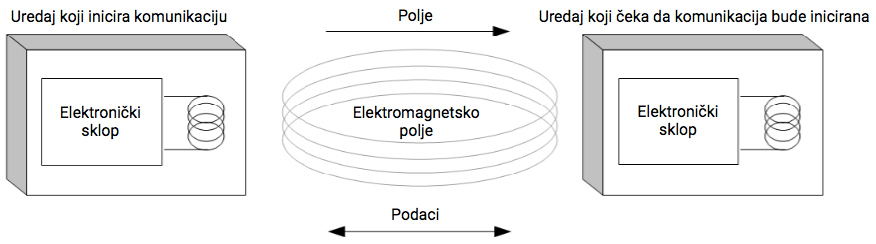
\includegraphics[height=4cm,keepaspectratio=true]{nfc_diagram}
 \caption{Komunikacija dva NFC ure\dj aja \cite{nfc_techonology}}
 \label{fig:nfc_arhitektura}
	\end{center}
\end{figure}

NFC ure\dj aji implementiraju dvije specifikacije i njihova funkcionalnost ovisi o tome po kojoj specifikaciji su izra\dj eni:

\begin{itemize}
	\item ISO/IEC 14443
	\begin{itemize}
		\item Definira memoriju NFC ure\dj aja
		\item Ure\dj aj je napravljen samo po ovoj specifikaciji je pasivni ure\dj aj i on ne mo\v{z}e inicirati komunikaciju (npr. naljepnica)
		
	\end{itemize}
	\item ISO/IEC 18092-3
	
	\begin{itemize}
		\item Definira elektromagnetsku komunikaciju (modulacije, kodiranje, inicijaliziaciju...)
		\item Ovi ure\dj aji implementiraju i ISO/IEC 14443 specifikaciju i oni su aktivni ure\dj aji
	\end{itemize}
\end{itemize}

Nadalje, ovisno o vrstama NFC ure\dj aja koji komuniciraju, komunikacija se dijeli na pasivnu i na aktivnu.


\subsection{Aktivna komunikacija}

Aktivna NFC komunikacija ozna\v{c}ava komunikaciju u dva smjera izme\dj u dva NFC ure\dj aja koji imaju vlastite izvore napajanja i napravljeni su po specifikaciji ISO/IEC 18000-3. Komunikacija se vr\v{s}i tako da ure\dj aj koji \v{z}eli poslati poruku aktivira svoje magnetsko polje preko kojega se poruka po\v{s}alje te ga deaktivira kada \v{z}eli primiti poruku. Ovakva komunikacija zahtjeva dodatnu logiku koja definira pravila komunikacije.

Aktivni NFC ure\dj aji se po arhitekturi dijele na \cite{nfc_types}:

\begin{itemize}
	\item NFC-A ure\dj aje
	\begin{itemize}
		\item Millerovo enkodiranje
		\item ASK modulacija 100%
		\item Brzina prijenosa 106 kb/s
	\end{itemize}

	\item NFC-B ure\dj aje
	\begin{itemize}
		\item Manchester enkodiranje
		\item ASK modulacija 10%
		\item Brzina prijenosa 106 kb/s
	\end{itemize}

	\item NFC-F (FeliCa) ure\dj aje
	\begin{itemize}
		\item Vrsta RFID protokola koja je jako sli\v{c}na NFC-u pa spada u istu kategoriju
		\item Razvijena je u Japanu gdje ima jako \v{s}iroku primjenu (najra\v{s}irenija je u kod prijevozni\v{c}kih karata)
		\item  Brzina prijenosa 212 kb/s
	\end{itemize}
\end{itemize}


\subsection{Pasivna komunikacija}

Pasivna komunikacija se vr\v{s}i izme\dj u aktivnog i pasivnog ure\dj aja, na na\v{c}in da aktivni ure\dj aj \v{s}alje signal nosioc kroz svoje elektromagnetsko polje \cite{nfc_arhitektura}. Ukoliko je pasivni ure\dj aj u dometu polje \'{c}e inducirati napon u njegovoj zavojnici te \'{c}e biti u stanju modulirati postoje\'{c}e polje, koriste\'{c}i ASK (amplitude-shift keying) modulaciju. To je znak aktivnom ure\dj aju da je komunikacija ostvarena. Nadalje, aktivni ure\dj aj pita pasivni koju vrstu komunikacije koristi (npr. komunikacija mo\v{z}e biti enkriptirana - koristi se kod pla\'{c}anja kreditnim karticama), te ovisno o odgovoru \v{s}alje odgovaraju\'{c}e zahtjeve za \v{c}itanjem memorije, \v{s}to mu pasivni i pru\v{z}a, nakon \v{s}to ih uspje\v{s}no validira.



Tipovi pasivnih NFC ure\dj aja uklju\v{c}uju \cite{nfc_pasivni}:

\begin{itemize}
	\item Tip 1
	\begin{itemize}
		\item Brisanje i \v{c}itanje memorije
		\item Mogu se konfigurirati da se mogu samo \v{c}itati
		\item Memorija: 96 B do 2kB
	\end{itemize}

	\item Tip 2
	\begin{itemize}
		\item Brisanje i \v{c}itanje memorije
		\item Mogu se konfigurirati da se mogu samo \v{c}itati
		\item Memorija: 48 B do 2kB
	\end{itemize}

	\item Tip 3
	\begin{itemize}
		\item Mogu ih \v{c}itati samo NFC-F ure\dj aji
		\item Ili konfigurabilni (\v{c}itanje i pisanje) ili samo za \v{c}itanje
		\item  Memorija varijabilna, teoretski mo\v{z}e biti do 1MB
	\end{itemize}

	\item Tip 4
	\begin{itemize}
		\item Ili konfigurabilni (\v{c}itanje i pisanje) ili samo za \v{c}itanje
		\item Memorija do 32 KB
	\end{itemize}
\end{itemize}


\section{Primjena}

Razvoj dana\v{s}nje tehnologije pru\v{z}a \v{c}ovje\v{c}anstvu sve opremljenije i prenosivije svakodnevne ure\dj aje. Samim time se je pojavila potreba za protokolom \v{c}ija \'{c}e primjena biti \v{s}to br\v{z}e i jednostavnije  prenjeti informacije sa ure\dj aja na ure\dj aj u kratkom dometu. Niska cijena, mogu\'{c}nost rada bez izvora energije i intinuitivnost kori\v{s}tenja (potrebno je samo prisloniti jedan NFC ure\dj aj o drugi) omogu\'{c}ava \v{s}iroku primjenu NFC-a, a neke njih uklju\v{c}uju:

\begin{itemize}
	\item Beskontaktno pla\'{c}anje kreditnim karticama ili pametnim telefonima
	\item Otklju\v{c}avanje ranih ure\dj aja (ra\v{c}unala, automobila, brava...)
	\item Razmjena vizitki
	\item \v{c}itanje konfiguracije WiFi mre\v{z}e
	\item Vo\dj enje \v{c}ita\v{c}a na internetsku poveznicu
	\item Ulaznice za razne doga\dj aje
\end{itemize}

Za potrebe ovog projekta kori\v{s}tene su NFC naljepnice kupljene preko internetske trgovine WhizTags \cite{whiztags}, prikazane na slici  ~\ref{fig:whiztags}.

\begin{figure}[!htbp]
	\begin{center}
 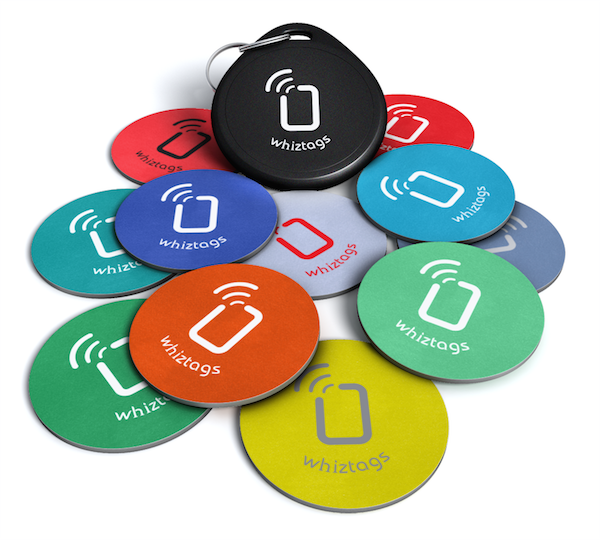
\includegraphics[height=8cm,keepaspectratio=true]{NTAG2161}
 \caption{Kori\v{s}tene NFC naljepnice}
 \label{fig:whiztags}
	\end{center}
\end{figure}

Specifikacija naljepnice:

\begin{itemize}
	\item NATG 216 NFC modul \cite{nat_modul}
	\item 888 B memorije
	\item Samoljepljivost
	\item Vodootpornost
\end{itemize}











